%\documentclass[dvips, intlimits, 8pt, unicode]{beamer} %для tex -> dvi -> ps -> pdf
\documentclass[pdf, 10pt, unicode,aspectratio=169]{beamer} %Для Latex2Pdf  tex -> pdf
% Для печати
%\documentclass[handout, pdf, 10pt, unicode]{beamer} %Для Latex2Pdf  tex -> pdf
%В качестве размера лучше использовать 9pt
%dvips нужно использовать только если использовать построение слайдов через PostScript
%intlimits - стиль для пределов интегралов (по желанию)
%unicode - обязательно
%Пакеты для русского языка
\usepackage[T2A]{fontenc}
\usepackage[utf8]{inputenc}
\usepackage[english,russian]{babel}
%
%% Для печати 2 слайда на страницу
%\usepackage{pgfpages}
%\mode<handout>{\setbeamercolor{background canvas}{bg=black!2}}
%\pgfpagesuselayout{2 on 1}[a4paper,border shrink=5mm]
%
%Пакет для вставки рисунков
\usepackage{graphicx}
%\usepackage[font=small]{caption,subfig}

\usepackage{times}
\usepackage{mathptmx}

\IfFileExists{pscyr.sty}
{
	% Хак с шрифтами
	\usepackage{times}
	\usepackage{mathptmx}
	\usepackage{pscyr}
	\def\rmdefault{ftm}
	\def\sfdefault{ftx}
	\def\ttdefault{fer}
	\DeclareMathAlphabet{\mathbf}{OT1}{ftm}{bx}{it} % bx/it or bx/m
}
% else
{
	\typeout{RFDstyle message: no PScyr, shall do without...}
}


\def\rmdefault{ftm}
\def\sfdefault{ftx}
\def\ttdefault{fer}
\DeclareMathAlphabet{\mathbf}{OT1}{ftm}{bx}{it} % bx/it or bx/m

%AMS TEX значки и пр.
\usepackage{amsfonts}
\usepackage{amsbsy}
\usepackage{amssymb}
\usepackage{amsthm}
\usepackage{multirow}
\usepackage{multicol}
\usepackage{verbatim}
\usepackage{makecell}
\usepackage{wrapfig}
\usepackage{subcaption}

%Векторная графика
\usepackage{tikz}
\usetikzlibrary{decorations.pathreplacing}

%\hypersetup{colorlinks=true}
\def\dfrac#1#2{\displaystyle{\frac{#1}{#2}}}
\def\Div{\mathop{\rm div}\nolimits}
\def\const{\mathop{\rm const}\nolimits}
\def\N{{\bf N}}
\def\q{{\bf q}}
\def\U{{\bf U}}
\def\F{{\bf F}}
\def\p{{\bf p}}
\def\eps{\varepsilon}
%\def\Bold#1{{\em #1}}
\def\Bold#1{{\bfseries #1}}
\def\Emph#1{{\bfseries #1}}
\def\Blue#1{\textcolor{blue}{#1}}
\def\dist{\mathop{\rm dist}\nolimits}

\newtheorem{defin}{Определение}


%разные пакеты
%\usepackage[mathscr]{eucal}
%\usepackage{cite}
%\usepackage{dsfont}
%\usepackage{indentfirst}

%Привычный шрифт для математических формул
\usefonttheme[onlymath]{serif}

%Нужно включать, если используется "тема" (стиль оформления) по умолчанию
%\usepackage{beamerthemesplit}

%Общий стиль ("тема") оформления слайдов
%Можно выбрать любую тему в \localtexmf\tex\latex\beamer\themes\theme\
%и ее имя подставить в качестве аргумента в \usetheme
%Требование: черные буквы на белом фоне
%\usetheme{Warsaw}
\usetheme{default}

%\setbeamertemplate{headline}{%
%\begin{beamercolorbox}{section in head/foot}
%{\ }\hfill\includegraphics[scale=0.08]{rfd-logo}\hskip2pt{\ }\vskip-21pt
%\end{beamercolorbox}%
%}
\setbeamertemplate{headline}{%
\begin{beamercolorbox}{section in head/foot}
{\ }\hfill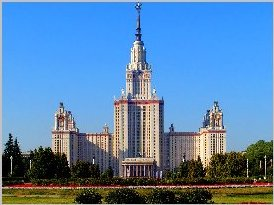
\includegraphics[scale=0.08]{msu.jpg}\hskip2pt{\ }\vskip-21pt
\end{beamercolorbox}%
}

% Сюда вствить ФИО и номер группы
\def\FullName{Федотов Иван Андреевич}
\def\ShortName{Федотов И. А.}
\def\Group{610}
\def\PaperType{Дипломная работа}


\setbeamertemplate{footline}{%
\begin{beamercolorbox}{section in head/foot}
\vskip1pt{\ }\hskip1pt%
\ShortName\hfill{}\PaperType%
\hskip1pt{\ }\vskip1pt%
\end{beamercolorbox}%
}

%\setbeamercolor{normal text}{bg=blue!4}

% Удаляем навигационную панель
\setbeamertemplate{navigation symbols}{}

% Устанавливаем поля (по умолчнанию - 1 см)
\setbeamersize{text margin left=0.5cm, text margin right=0.25cm}

%Более крупный шрифт для подзаголовков титульного листа
\setbeamerfont{institute}{size=\normalsize}

%Задание команды (\bluetext) для выделения конкретным (синим) цветом
%\alert - выделение цветом выбранной "темы"
\setbeamercolor{bluetext_color}{fg=blue}
\newcommand{\bluetext}[1]{{\usebeamercolor[fg]{bluetext_color}#1}}

%Если используется последовательное появление пунктов списков на слайде
%(не злоупотребляйте в слайдах), чтобы
%еще непоявившиеся пункты были все-таки немножко видны.
\setbeamercovered{transparent}

% Путь к файлам с иллюстрациями
\graphicspath{{./src/pics/}}

\def\MyColorBox#1{{%
\centering
\textcolor{blue}{%
\fbox{\textcolor{black}{%
\parbox{0.98\textwidth}{\centering\parbox{0.97\textwidth}{%
\noindent\strut{}%
#1\strut}}}}}%
}}


\title{Распределённая система хранения состояния на основе алгоритма для решения задач консенсуса в распределенной среде ненадежных узлов}

\author[\FullName]{\FullName \newline студент \Group{} группы}

 \institute{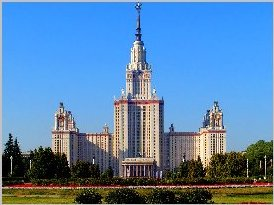
\includegraphics[scale=0.3]{msu.jpg} \\[2ex] 
  Научный руководитель --- д.\,ф.-м.\,н., профессор \,{К.Ю. Богачев }\\ }
  \date{     Москва,     2024 г. }

\begin{document}

\begin{frame}[plain]
\titlepage
\end{frame}

%%%%%%%%%%%%%%%%%%%%%%%%%%%%%%%%%%%%%%%%%%%%%%%%%%%%%%%%%%%%%%%%%%%%



%%%%%%%%%%%%%%%%%%%%%%%%%%%%%%%%%%%%%%%%%%%%%%%%%%%%%%%%%%%%%%%%%%%
\begin{frame}
\frametitle{Введение.}
% \cite{tNavigatorManual}

\begin{wrapfigure}[12]{r}{0.5\linewidth} 
  \begin{minipage}{1\textwidth}
    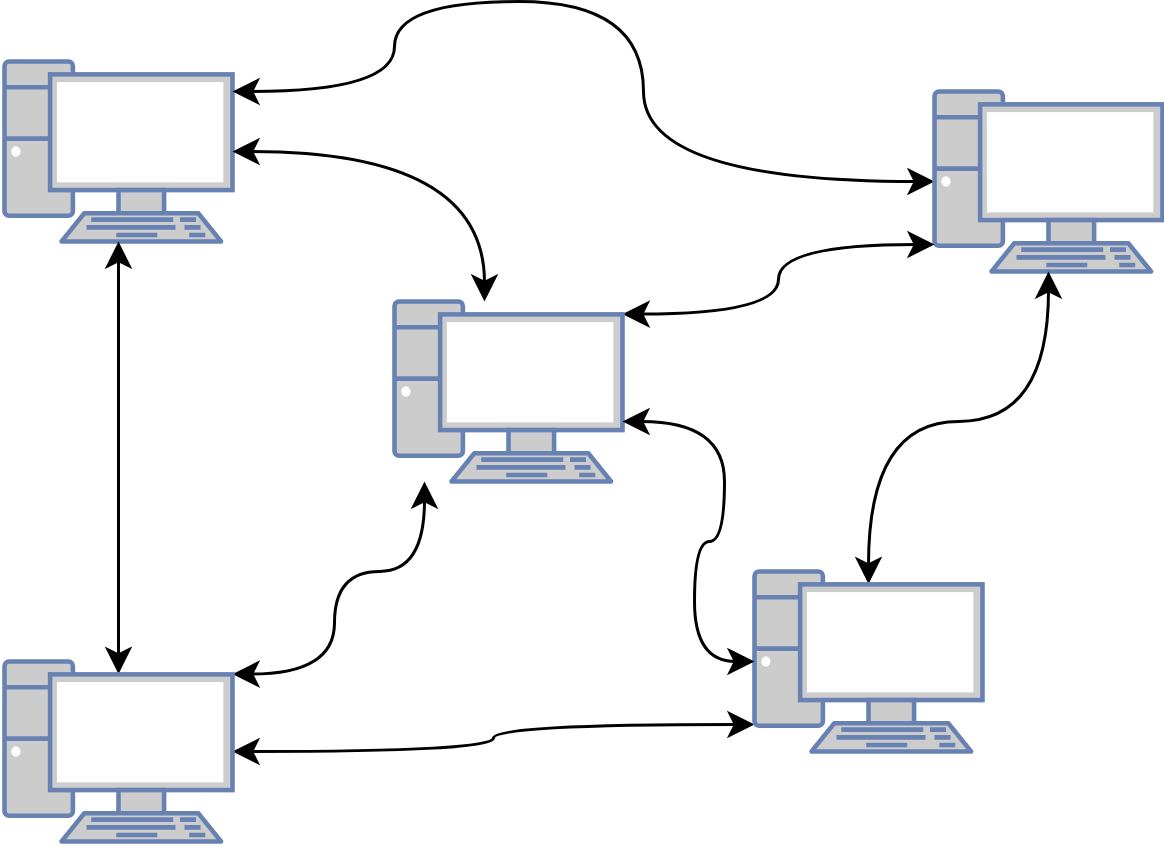
\includegraphics[width=0.4\linewidth]{dist_sys.png}
    \end{minipage}
\end{wrapfigure}

\textit{Распределенная система} - это набор независимых компьютеров (узлов), которые представляются пользователю как единая согласованная система.
\\\

\textit{Задача достижения консенсуса} - это задача получения согласованного значения группой участников, члены которой называются узлами, в ситуации, когда возможны отказы отдельных участников, предоставления им некорректной информации или искажения переданных значений средой передачи данных.

\end{frame}
%%%%%%%%%%%%%%%%%%%%%%%%%%%%%%%%%%%%%%%%%%%%%%%%%%%%%%%%%%%%%%%%%%%

%%%%%%%%%%%%%%%%%%%%%%%%%%%%%%%%%%%%%%%%%%%%%%%%%%%%%%%%%%%%%%%%%%%
\begin{frame}
\frametitle{Постановка задачи.}
% \cite{tNavigatorManual}

Целью данной дипломной работы является реализация на C++ программы создания распределённой системы на основе одного из алгоритмов консенсуса и существующей централизованной системы. 

\end{frame}
%%%%%%%%%%%%%%%%%%%%%%%%%%%%%%%%%%%%%%%%%%%%%%%%%%%%%%%%%%%%%%%%%%%


%%%%%%%%%%%%%%%%%%%%%%%%%%%%%%%%%%%%%%%%%%%%%%%%%%%%%%%%%%%%%%%%%%%
\begin{frame}
	\frametitle{Задача принятия консенсуса}

Консенсус должен удовлетворять следующим условиям:
\begin{enumerate}
\item \textbf{Согласованность}: все корректные работающие узлы принимают одно и то же значение (\textit{"свойство безопасности"});
\item \textbf{Корректность}: выбранное значение должно быть одним из тех, которое было предложено каким-либо корректно работающим узлом (\textit{"свойство нетривиальности"});
\item \textbf{Конечность}: каждый корректно работающий узел должен делать выбор за конечное количество шагов (\textit{"свойство завершённости"});
\end{enumerate}


Теорема Фишера, Линча и Патерсона гласит, что не существует асинхронного детерминированного алгоритма принятия консенсуса, который был бы устойчив к выходу из строя одного узла и гарантировал бы все свойства консенсуса \cite{Theorem_FLP}.

\emph{Асинхронизм} означает, что нельзя достоверно различить работает ли узел медленно, или долго идет сообщение, или же отказал узел

\end{frame}
%%%%%%%%%%%%%%%%%%%%%%%%%%%%%%%%%%%%%%%%%%%%%%%%%%%%%%%%%%%%%%%%%%%


%%%%%%%%%%%%%%%%%%%%%%%%%%%%%%%%%%%%%%%%%%%%%%%%%%%%%%%%%%%%%%%%%%%
\begin{frame}
	\frametitle{Возможные типы ошибок}

В контексте задачи консенсуса существуют разные типы ошибок:
\begin{enumerate}
\item \textbf{Остановка с сигналом}: узел прекращает работу, а затем сообщает другим узлам о своем сбое. 

\item \textbf{Остановка}: узел преждевременно прекращает какую-либо активность, несмотря на то, что до остановки он работал полностью корректно.

\item \textbf{Потери сообщений}: при отсылке и при отправлении сообщений могут происходить потери сообщений, противоположная сторона никак не может узнать, что сообщение, было потеряно;

\item \textbf{Византийския ошибка}: наиболее сложный тип ошибки, процесс начинает себя вести некорректно. Например, посылать лишние или противоречивые сообщения, не работать какое-то время и так далее.
\end{enumerate}

\end{frame}
%%%%%%%%%%%%%%%%%%%%%%%%%%%%%%%%%%%%%%%%%%%%%%%%%%%%%%%%%%%%%%%%%%%


%%%%%%%%%%%%%%%%%%%%%%%%%%%%%%%%%%%%%%%%%%%%%%%%%%%%%%%%%%%%%%%%%%%
\begin{frame}
	\frametitle{CAP-теорема}

CAP-теорема утверждает, что невозможно создать распределенную систему, которая будет одновременно удовлетворять
трём следующим свойствам:



\begin{minipage}[c]{0.45\linewidth}
\begin{itemize}
\item \textbf{Согласованности} - во всех узлах в один момент времени данные не противоречат друг другу
\item \textbf{Доступности} - любой запрос к распределённой системе завершается откликом, однако без гарантии, что ответы всех узлов системы совпадают
\item \textbf{Устойчивости к разделению} - расщепление распределённой системы на несколько изолированных секций не приводит к некорректности отклика от каждой из секций
\end{itemize}
\end{minipage}
\begin{minipage}[c]{0.53\linewidth}
\begin{figure}[H]
    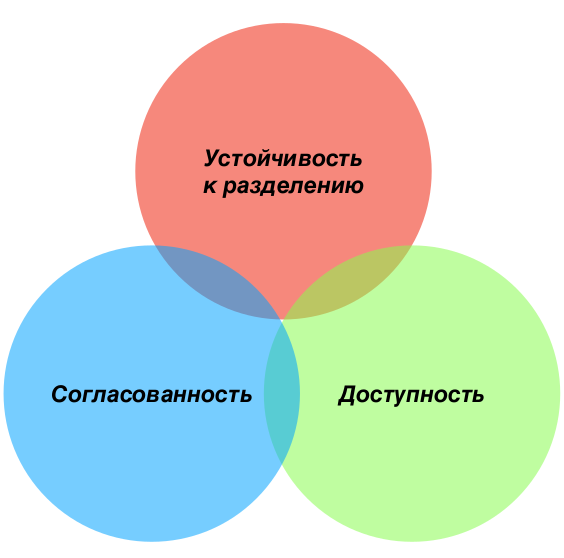
\includegraphics[width=0.8\textwidth]{CAP_t.png}
    %\caption*{Многоствольная скважина в tNavigator}
\end{figure}
\end{minipage}

\end{frame}
%%%%%%%%%%%%%%%%%%%%%%%%%%%%%%%%%%%%%%%%%%%%%%%%%%%%%%%%%%%%%%%%%%%


%%%%%%%%%%%%%%%%%%%%%%%%%%%%%%%%%%%%%%%%%%%%%%%%%%%%%%%%%%%%%%%%%%%
\begin{frame}
\frametitle{Распределенный конечный автомат}


\vspace{-15pt}

\begin{wrapfigure}{r}{0.55\textwidth}
\vspace{-25pt}
\hspace{-20pt}
%\begin{center}
\includegraphics[width=0.55\textwidth]{state_machine.png}
%\end{center}
%\vspace{-20pt}
\caption{Архитектура системы с использованием распределенного конечного автомата.}
\end{wrapfigure}

%\begin{figure}[H]
%\centering
%\includegraphics[width=0.5\textwidth]{src/pics/state_machine.png}
%\label{fig:state_machine}
%\end{figure}

 Алгоритм принятия консенсуса управляет реплицированным журналом, который содержит команды для конечного автомата, пришедшие от клиентов. 

Конечные автоматы с идентичным состоянием выполняют идентичную последовательность команд из реплицированного журнала, поэтому они порождают одинаковые выходные данные.

\end{frame}
%%%%%%%%%%%%%%%%%%%%%%%%%%%%%%%%%%%%%%%%%%%%%%%%%%%%%%%%%%%%%%%%%%%


%%%%%%%%%%%%%%%%%%%%%%%%%%%%%%%%%%%%%%%%%%%%%%%%%%%%%%%%%%%%%%%%%%%
\begin{frame}
\frametitle{Различные алгоритмы консенсуса}

%При построении распределённой системы, нужно отказаться от одного из свойств, перечисленных в CAP теореме.
%Если отказаться от устойчивости к разделению, то такая система потеряет одно из своих основных преимуществ, а именно отказоустойчивость, так как при отделении даже одного узла, система не сможет корректно обработать ни один запрос.
%Свойство согласованности игнорировать полностью также нельзя, так как в таком случае распределённая система может разделиться на несколько самостоятельных частей, никак не согласовывающих ответы на запросы. 
%Если же рассматривать оставшиеся варианты, можно разделить алгоритмы следующим образом:

\begin{figure}[H]
\centering
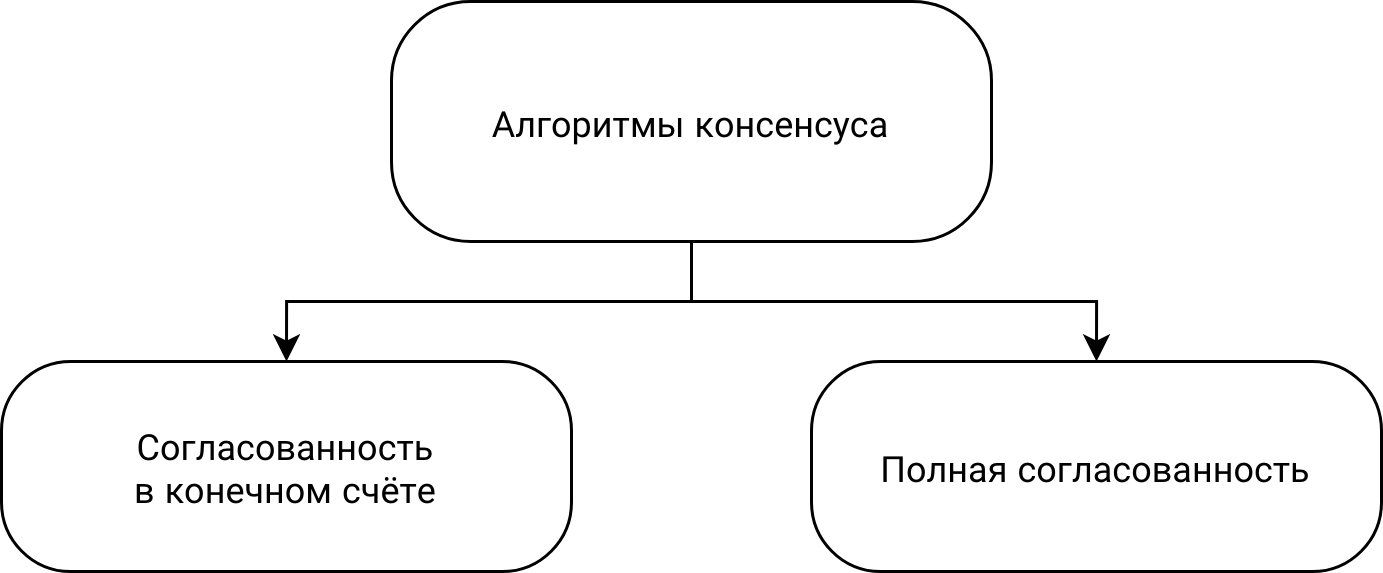
\includegraphics[width=0.6\textwidth]{src/pics/consensus_types_1.png}
\label{fig:consensus_types_1}
\end{figure}

\emph{Полная согласованность} - это в точности то, что определяется в CAP теореме.\\\

\emph{Согласованность в конечном итоге} - это свойство, при котором гарантируется, что в отсутствии изменений данных, через какой-то промежуток времени после последнего обновления ("в конечном счёте") все запросы будут возвращать последнее обновлённое значение.

\end{frame}
%%%%%%%%%%%%%%%%%%%%%%%%%%%%%%%%%%%%%%%%%%%%%%%%%%%%%%%%%%%%%%%%%%%


%%%%%%%%%%%%%%%%%%%%%%%%%%%%%%%%%%%%%%%%%%%%%%%%%%%%%%%%%%%%%%%%%%%
\begin{frame}
\frametitle{Алгоритмы с согласованностью в конечном итоге}

\begin{figure}[H]
\centering
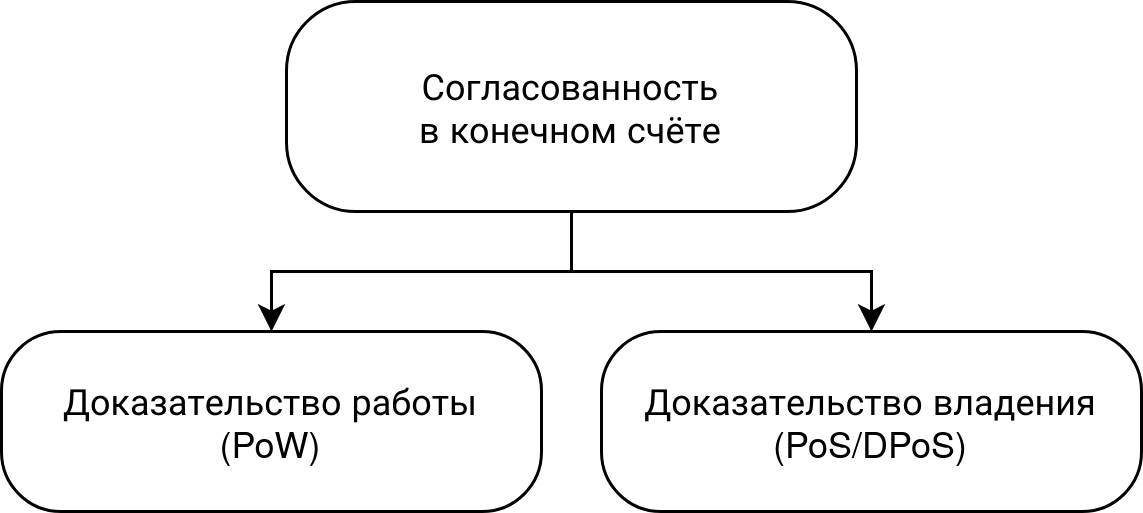
\includegraphics[width=0.8\textwidth]{src/pics/consensus_types_2.png}
\caption{Примеры алгоритмов, согласованных в конечном итоге.}
\label{fig:consensus_types_2}
\end{figure}

\end{frame}
%%%%%%%%%%%%%%%%%%%%%%%%%%%%%%%%%%%%%%%%%%%%%%%%%%%%%%%%%%%%%%%%%%%


%%%%%%%%%%%%%%%%%%%%%%%%%%%%%%%%%%%%%%%%%%%%%%%%%%%%%%%%%%%%%%%%%%%
\begin{frame}
\frametitle{Алгоритмы с полной согласованностью}

\begin{figure}[H]
\centering
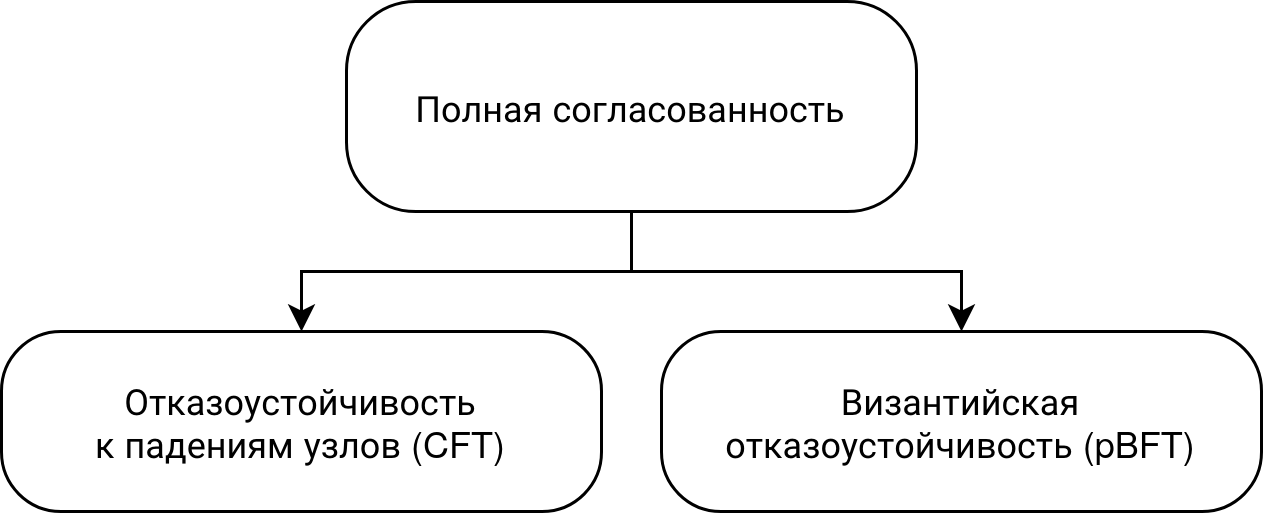
\includegraphics[width=0.85\textwidth]{src/pics/consensus_types_3.png}
\caption{Деление алгоритмов с полной согласованностью.}
\label{fig:consensus_types_3}
\end{figure}

\end{frame}
%%%%%%%%%%%%%%%%%%%%%%%%%%%%%%%%%%%%%%%%%%%%%%%%%%%%%%%%%%%%%%%%%%%


%%%%%%%%%%%%%%%%%%%%%%%%%%%%%%%%%%%%%%%%%%%%%%%%%%%%%%%%%%%%%%%%%%%
\begin{frame}
\frametitle{Сравнение алгоритмов}
Как итог сравнения перечисленных алгоритмов можно составить таблицу характеристик:
\begin{itemize}
\item Согласованность - полная или в конечном счёте
\item Отказоустойчивость - количество единичных отказов узлов системы из $N$ узлов, после наступления которых сохраняется работоспособность системы в целом. 
\item Вычислительная сложность - оценка количества вычислений, требующихся для принятия консенсуса.
\item Масштабируемость - способность системы справляться с увеличением нагрузки с увеличением количества узлов.
\end{itemize}

\begin{table}[H]
\begin{center}
\begin{tabular}{|c|c|c|c|c|}
\hline
Свойство & PoW & PoS/DPoS & pBFT & Raft \\
\hline
Согласованность & \multicolumn{2}{c}{В конечном счёте} & \multicolumn{2}{|c|}{Полная}    \\
\hline
Отказоустойчивость & \multicolumn{2}{c|}{$N/2$} & $N/3$ & $N/2$  \\
\hline
Вычислительная сложность  & Высокая & Низкая & \multicolumn{2}{c|}{Незначительная}  \\
\hline
Масштабируемость & \multicolumn{2}{c|}{Высокая} & \multicolumn{2}{c|}{Низкая}  \\
\hline
\end{tabular}
\end{center}
\end{table} 

\end{frame}
%%%%%%%%%%%%%%%%%%%%%%%%%%%%%%%%%%%%%%%%%%%%%%%%%%%%%%%%%%%%%%%%%%%


%%%%%%%%%%%%%%%%%%%%%%%%%%%%%%%%%%%%%%%%%%%%%%%%%%%%%%%%%%%%%%%%%%%
\begin{frame}
\frametitle{Алгоритм Raft}

\begin{wrapfigure}{r}{0.3\textwidth}
%\vspace{-25pt}
%\hspace{-20pt}
%\begin{center}

\includegraphics[width=0.3\textwidth]{raft_pic.png}
%\end{center}
%\vspace{-20pt}
\end{wrapfigure}

Алгоритм Raft - это алгоритм консенсуса, разработанный для обеспечения надежности и отказоустойчивости в распределенных системах. Он основан на идее выбора лидера среди узлов системы, который затем координирует работу всех остальных узлов. Raft разбивает процесс выбора лидера и репликации данных на два независимых шага, что облегчает понимание и реализацию алгоритма. При помощи голосования и случайных таймаутов Raft выбирает лидера, который затем управляет репликацией данных и поддержанием консистентности. Алгоритм Raft обеспечивает высокую устойчивость к отказам узлов и позволяет системе продолжать работу при сбоях и разрывах связи. Данные, обслуживаемые кластером Raft, представляют собой лог, состоящий из записей. Когда пользователь хочет изменить данные, хранящиеся в кластере, он добавляет в лог новую запись с командой.

\end{frame}
%%%%%%%%%%%%%%%%%%%%%%%%%%%%%%%%%%%%%%%%%%%%%%%%%%%%%%%%%%%%%%%%%%%


%%%%%%%%%%%%%%%%%%%%%%%%%%%%%%%%%%%%%%%%%%%%%%%%%%%%%%%%%%%%%%%%%%%
\begin{frame}
\frametitle{Алгоритм Raft. Состояния.}


Каждый узел может находится в одном из 3-х состояний:
\begin{enumerate}
\item Лидер - обрабатывает все клиентские запросы, поддерживает актуальность лога.
\item Кандидат - состояние сервера, возможное только во время выбора нового лидера.
\item Ведомый - пассивный сервер, который только записывает новые записи в лог от лидера и перенаправляет все входящие запросы от клиентов на лидера.
\end{enumerate}

\begin{figure}[H]
\centering
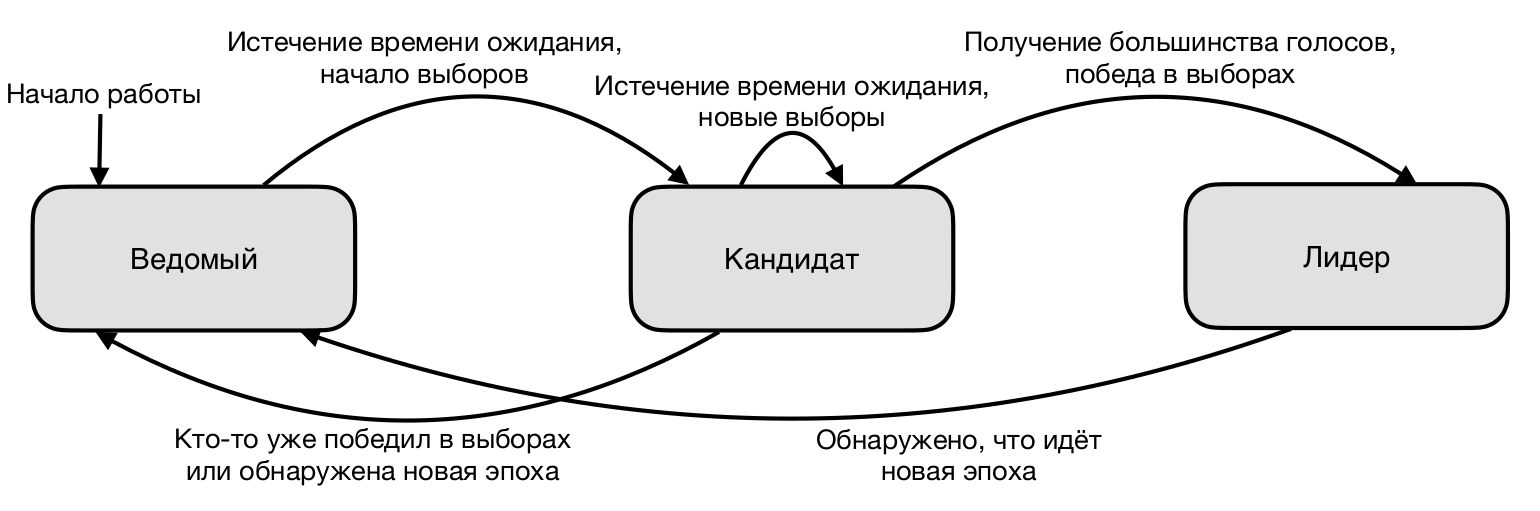
\includegraphics[width=0.95\textwidth]{src/pics/states.png}
\label{fig:states}
\end{figure}


\end{frame}
%%%%%%%%%%%%%%%%%%%%%%%%%%%%%%%%%%%%%%%%%%%%%%%%%%%%%%%%%%%%%%%%%%%


%%%%%%%%%%%%%%%%%%%%%%%%%%%%%%%%%%%%%%%%%%%%%%%%%%%%%%%%%%%%%%%%%%%
\begin{frame}
\frametitle{Алгоритм Raft. Эпохи.}


Raft делит время на отрезки произвольной длины, называемые эпохами. Каждая эпоха имеет монотонно возрастающий номер. 

\begin{figure}[H]
\centering
\vspace{0.4cm}
\hspace*{0.2cm}
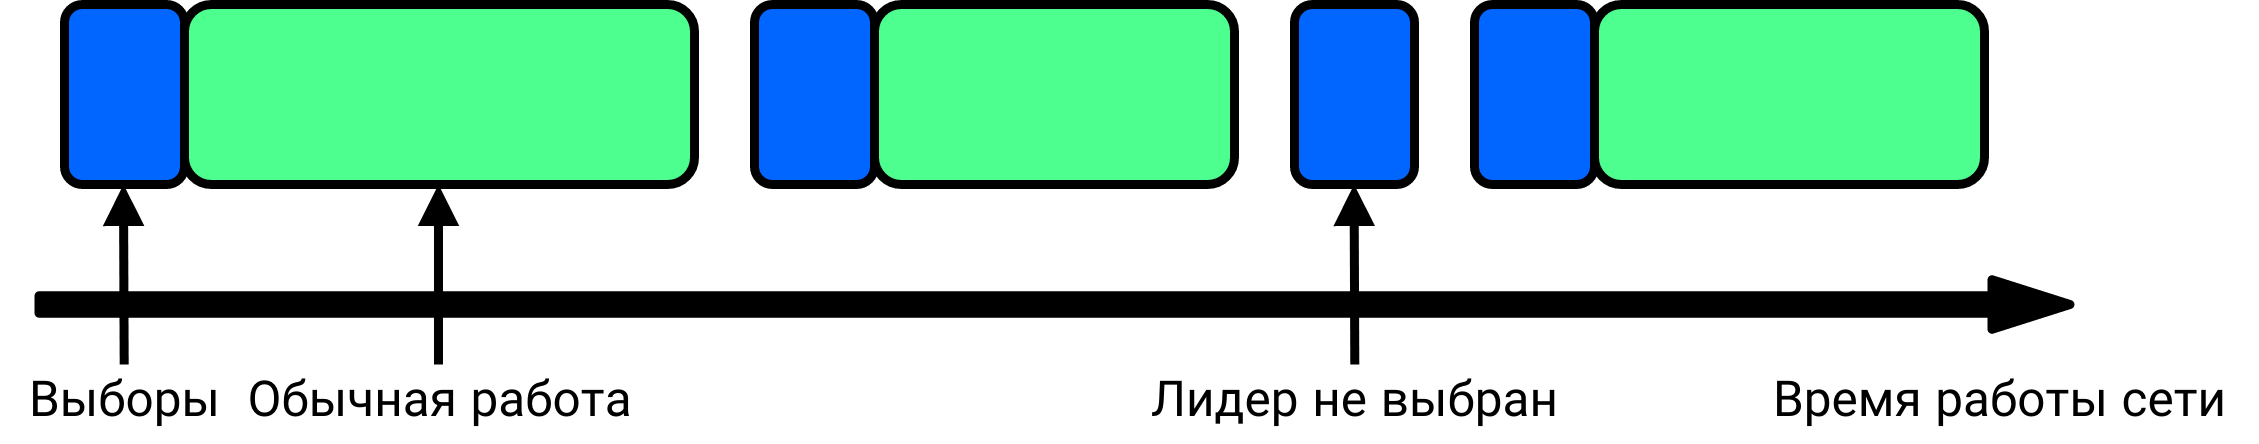
\includegraphics[width=0.95\textwidth]{src/pics/terms.png}
\caption{Время делится на эпохи, и каждая эпоха начинается с процедуры выборов лидера. После успешных выборов, лидер управляет системой до конца эпохи. Некоторые выборы заканчиваются неудачно, и в этом случае эпоха заканчивается без выбора лидера. Переходы между эпохами можно наблюдать в различные моменты времени на различных серверах.}
\label{fig:terms}
\end{figure}

\end{frame}
%%%%%%%%%%%%%%%%%%%%%%%%%%%%%%%%%%%%%%%%%%%%%%%%%%%%%%%%%%%%%%%%%%%


%%%%%%%%%%%%%%%%%%%%%%%%%%%%%%%%%%%%%%%%%%%%%%%%%%%%%%%%%%%%%%%%%%%
\begin{frame}
\frametitle{Алгоритм Raft. Взаимодействие.}

Серверы в Raft взаимодействуют посредством обмена запросами и ответами. Базовый алгоритм использует всего два вида вызовов: 
\begin{itemize}
\item \emph{RequestVote} используется кандидатами во время выборов. Запрос содержит номер эпохи кандидата и метаданные о логе кандидата, более подробно рассмотренные далее. Ответ содержит номер эпохи отвечающего сервера и значение «true», если сервер голосует за кандидата; «false», если сервер голосует против кандидата.
\item \emph{AppendEntries} используется лидером для репликации лога, а также для механизма heartbeat. Запрос содержит номер эпохи лидера, коллекцию записей, которые нужно добавить в лог (или пустую коллекцию в случае heartbeat), некоторые метаданные о логе лидера, также подробнее рассмотренные далее. Ответ содержит номер эпохи ведомого и значение «true», если ведомый успешно добавил записи в свой лог; «false», если добавить записи в лог не удалось.
\end{itemize}


\end{frame}
%%%%%%%%%%%%%%%%%%%%%%%%%%%%%%%%%%%%%%%%%%%%%%%%%%%%%%%%%%%%%%%%%%%


%%%%%%%%%%%%%%%%%%%%%%%%%%%%%%%%%%%%%%%%%%%%%%%%%%%%%%%%%%%%%%%%%%%
\begin{frame}
\frametitle{Алгоритм Raft. Процедура выборов 1.}

%\begin{figure}[H]
%	\centering
%	\begin{tabular}{cc}
%		\includegraphics[width = 0.35\linewidth]{elec_1} &
%		\includegraphics[width = 0.35\linewidth]{elec_2}\\
%
%Система находился в эпохе номер 4,\\ с лидером Л4, который рассылает \\контрольные сообщения ведомым.  &
%Лидер Л4 отказывает. \\
%Без контрольного сообщения от лидера,\\ таймеры ведомых не обновляются\\ и начнётся голосование.
%	\end{tabular}
%	%\caption{Пример сетки и свойства на этой сетке.}
%\end{figure}

%\begin{wrapfigure}{c}{0.8\textwidth}
%\hfill
%\begin{minipage}{0.4\linewidth}
%\center{\includegraphics[width=0.8\linewidth]{src/pics/elec_1.png}} 
%\begin{small}
%Система находился в эпохе номер 4, с лидером Л4, который рассылает контрольные сообщения ведомым. 
%\end{small}
%\end{minipage}
%\begin{minipage}{0.4\linewidth}
%\center{\includegraphics[width=0.8\linewidth]{src/pics/elec_2.png}} 
%\begin{small}
%Лидер Л4 отказывает. Без контрольного сообщения от лидера, таймеры ведомых не обновляются и начнётся голосование.
%\end{small}
%\end{minipage}
%\end{wrapfigure}

\begin{figure}[H]
\begin{minipage}[h]{0.49\linewidth}
\center{\includegraphics[width=0.7\linewidth]{src/pics/elec_1.png}} 
\begin{small}
Система находился в эпохе номер 4, с лидером Л4, который рассылает контрольные сообщения ведомым.  \\
\end{small}
\end{minipage}
\hfill
\begin{minipage}[h]{0.49\linewidth}
\center{\includegraphics[width=0.7\linewidth]{src/pics/elec_2.png}} 
\begin{small}
СЛидер Л4 отказывает. Без контрольного сообщения от лидера, таймеры ведомых не обновляются и начнётся голосование. \\
\end{small}
\end{minipage}
\end{figure}

\end{frame}
%%%%%%%%%%%%%%%%%%%%%%%%%%%%%%%%%%%%%%%%%%%%%%%%%%%%%%%%%%%%%%%%%%%


%%%%%%%%%%%%%%%%%%%%%%%%%%%%%%%%%%%%%%%%%%%%%%%%%%%%%%%%%%%%%%%%%%%
\begin{frame}
\frametitle{Алгоритм Raft. Процедура выборов 2.}


\begin{figure}[H]
\begin{minipage}[h]{0.49\linewidth}
\center{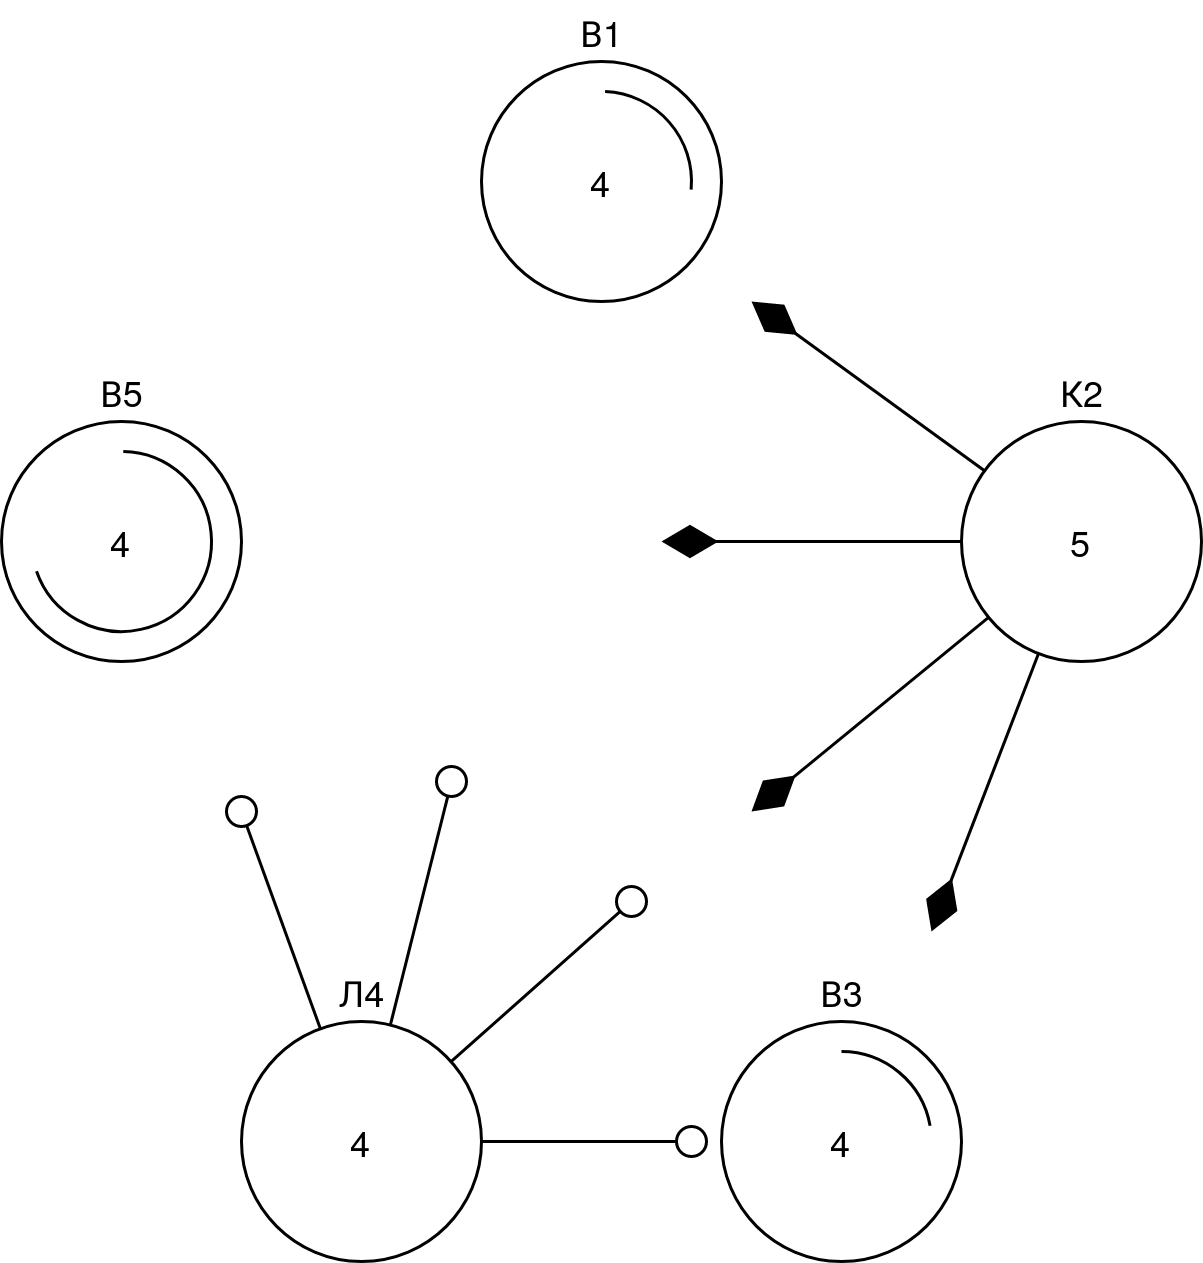
\includegraphics[width=0.7\linewidth]{src/pics/elec_3.png}} 
\begin{small}
Сервер К2 становится кандидатом, увеличивает номер своей эпохи, и отправляет всем серверам сообщение с началом голосования. В это же время сервер Л4 восстанавливается после сбоя, и посылает контрольное сообщение всем серверам для подтверждения своего лидерства \\
\end{small}
\end{minipage}
\hfill
\begin{minipage}[h]{0.49\linewidth}
\center{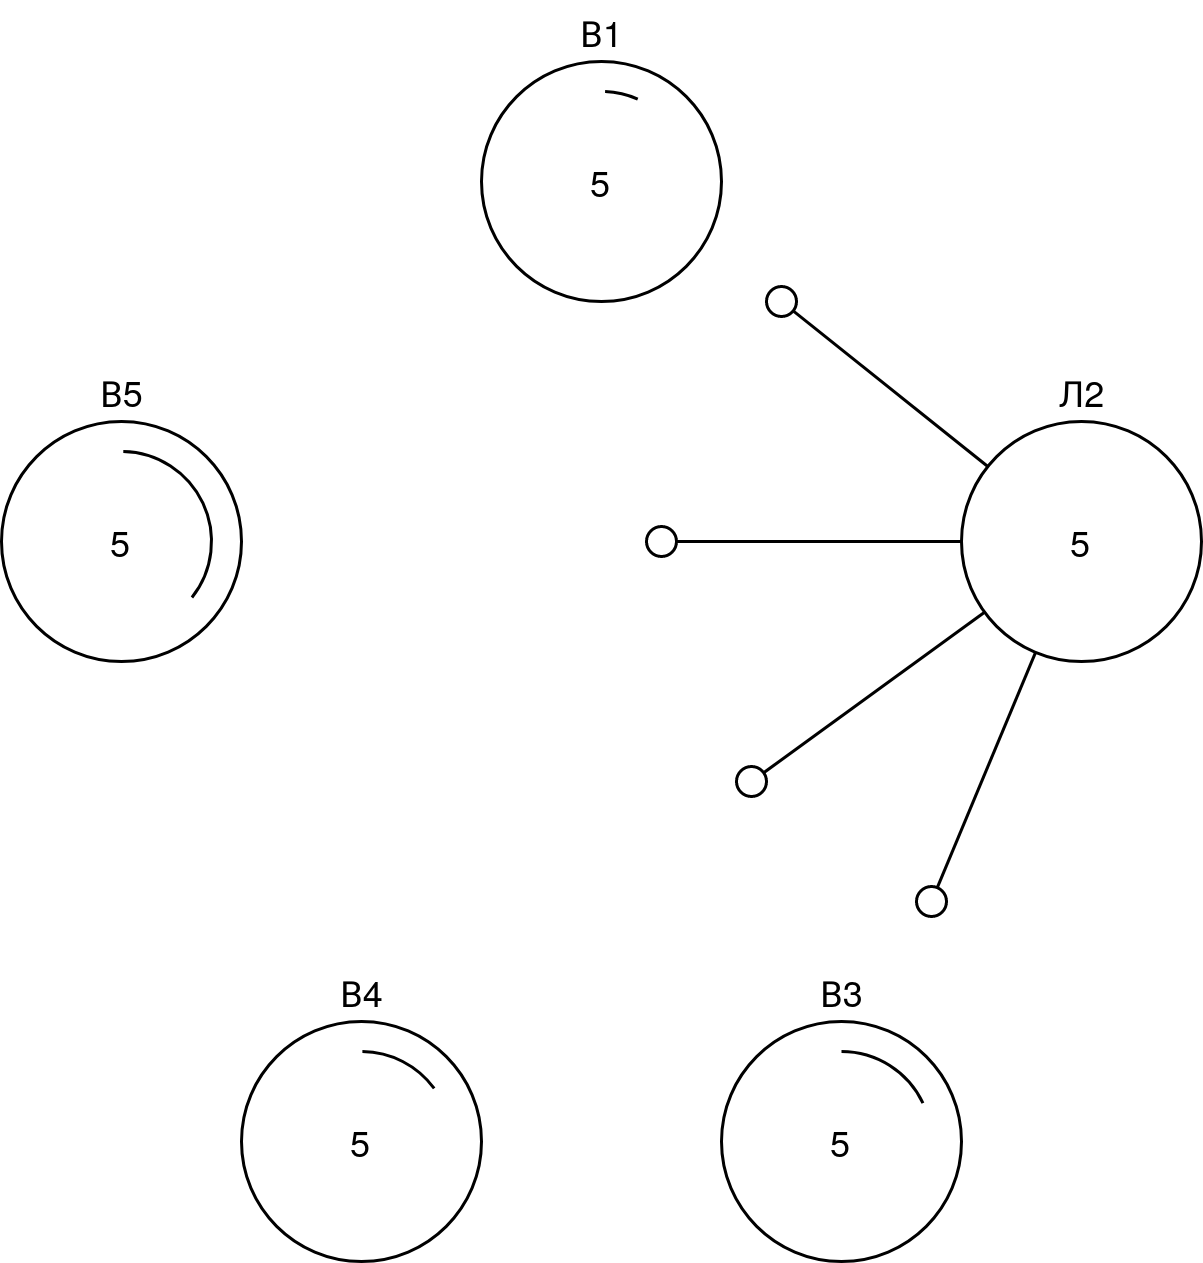
\includegraphics[width=0.7\linewidth]{src/pics/elec_4.png}} 
\begin{small}
Сервер К2, получив большинство голосов (от В1, В3, В5), становится лидером Л2. Л4, получив сообщение от Л2, отвергает его, так как его номер эпохи больше. Л4, получив от Л2 сообщение,
становится ведомым В4 с эпохой 5, так как обнаруживает, что его номер эпохи устарел \\
\end{small}
\end{minipage}
\end{figure}

\end{frame}
%%%%%%%%%%%%%%%%%%%%%%%%%%%%%%%%%%%%%%%%%%%%%%%%%%%%%%%%%%%%%%%%%%%


%%%%%%%%%%%%%%%%%%%%%%%%%%%%%%%%%%%%%%%%%%%%%%%%%%%%%%%%%%%%%%%%%%%
\begin{frame}
\frametitle{Алгоритм Raft. Реплицкация журнала}

\begin{wrapfigure}{r}{0.6\textwidth}
\vspace{-60pt}
%\hspace{-20pt}
%\begin{center}
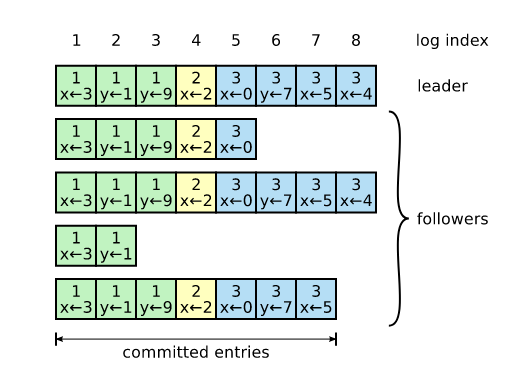
\includegraphics[width=0.6\textwidth]{log_1.png}
%\end{center}
%\vspace{-20pt}
\end{wrapfigure}

Журналы состоят из записей, которые нумеруются последовательно. Каждая запись содержит номер эпохи, в которой он был создан и команду для конечного автомата.

\end{frame}
%%%%%%%%%%%%%%%%%%%%%%%%%%%%%%%%%%%%%%%%%%%%%%%%%%%%%%%%%%%%%%%%%%%


%%%%%%%%%%%%%%%%%%%%%%%%%%%%%%%%%%%%%%%%%%%%%%%%%%%%%%%%%%%%%%%%%%%
\begin{frame}
\frametitle{Тесты}


\end{frame}
%%%%%%%%%%%%%%%%%%%%%%%%%%%%%%%%%%%%%%%%%%%%%%%%%%%%%%%%%%%%%%%%%%%


%%%%%%%%%%%%%%%%%%%%%%%%%%%%%%%%%%%%%%%%%%%%%%%%%%%%%%%%%%%%%%%%%%%
\begin{frame}
\frametitle{Заключение}

В рамках данной работы был разработан и реализован а языке C++ алгоритм построения распределенной системы на основе алгоритма консенсуса Raft.\\\

Используя написанный алгоритм, существующая централизованная система сервера лицензий была преобразована в распределённый сервер и внедрена в программный пакет геолого-гидродинамического моделирования tNavigator. 

\end{frame}
%%%%%%%%%%%%%%%%%%%%%%%%%%%%%%%%%%%%%%%%%%%%%%%%%%%%%%%%%%%%%%%%%%%


%%%%%%%%%%%%%%%%%%%%%%%%%%%%%%%%%%%%%%%%%%%%%%%%%%%%%%%%%%%%%%%%%%%
\begin{frame}
\begin{center}
\Huge{\Blue{Спасибо за внимание!}}
\end{center}
\end{frame}
%%%%%%%%%%%%%%%%%%%%%%%%%%%%%%%%%%%%%%%%%%%%%%%%%%%%%%%%%%%%%%%%%%%

%%%%%%%%%%%%%%%%%%%%%%%%%%%%%%%%%%%%%%%%%%%%%%%%%%%%%%%%%%%%%%%%%%%
\begin{frame}[fragile]

\ifx\undefined\BibEmph\def\BibEmph#1{#1}\else\fi
\ifx\undefined\href\def\href#1#2{#2}\else\fi
\ifx\undefined\url\def\url#1{\texttt{#1}}\else\fi
\ifx\undefined\urlprefix\def\urlprefix{URL: }\else\fi
\ifx\undefined\BibUrl\def\BibUrl#1{\urlprefix\url{#1}}\else\fi
\ifx\undefined\BibUrlDate\long\def\BibUrlDate#1{({%
\cyr\cyrd\cyra\cyrt\cyra\
\cyro\cyrb\cyrr\cyra\cyrshch\cyre\cyrn\cyri\cyrya}: #1)}\else\fi
\ifx\undefined\BibAnnote\long\def\BibAnnote#1{#1}\else\fi
%% 
\begin{thebibliography}{1}
\addcontentsline{toc}{section}{\bibname}
\def\selectlanguageifdefined#1{
	\expandafter\ifx\csname date#1\endcsname\relax
	\else\language\csname l@#1\endcsname\fi}
	

\bibitem{Geostatistics}
\selectlanguageifdefined{russian}
В.В. Демьянов, Е.А. Савельева \em Геостатистика: теория и практика\em. Наука. Москва. 2010.


\bibitem{tNavigatorManual}
\selectlanguageifdefined{english}
\BibEmph{tNavigator.}
tNavigator User Manual. 
\BibEmph{Rock Flow Dynamics. 2024.}

\bibitem{Theorem_FLP}
\selectlanguageifdefined{english}
\BibEmph M. Fisher, N. Lynch, M. Paterson
\em  Impossibility of Distributed Consensus with One Faulty Process\em.
\BibEmph ACM, Volume 32, Issue 2; 1985

\end{thebibliography}
\bibliographystyle{gost705}

\end{frame}
%%%%%%%%%%%%%%%%%%%%%%%%%%%%%%%%%%%%%%%%%%%%%%%%%%%%%%%%%%%%%%%%%%% 

\end{document}
